
Pasting  from other another section:

EUDAQ serves as a tool set and an integration layer for the user DAQ system(s), providing the communication protocols for them to participate in a common DAQ. 

EUDAQ is a modular cross platform data Acquisition System designed in the context of the \eudet test beam Telescopes. 
It consist of completely independent modules such as run-control, log-Collector, Data-Collector and Producer. 
The communication between individual modules is done via TCP/IP therefore it is possible to run each module on a separate PC. 


\begin{figure}[tb]
	\center
	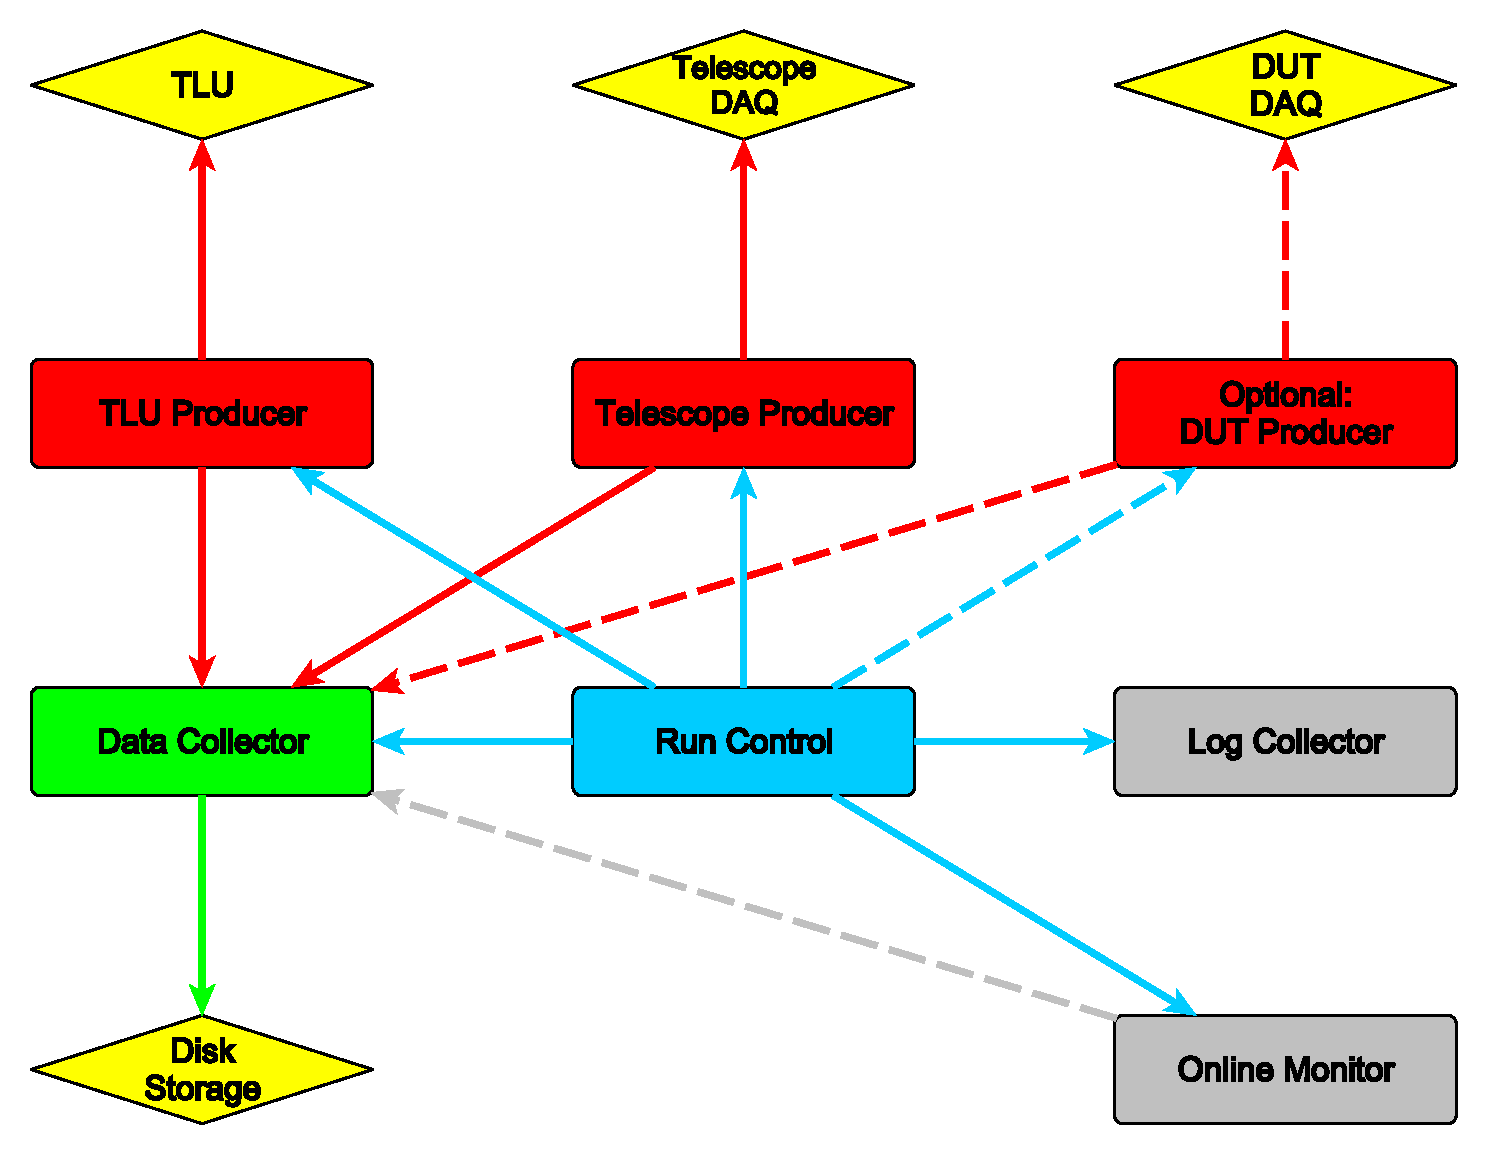
\includegraphics[width=.55\textwidth]{figures/eudaq}
	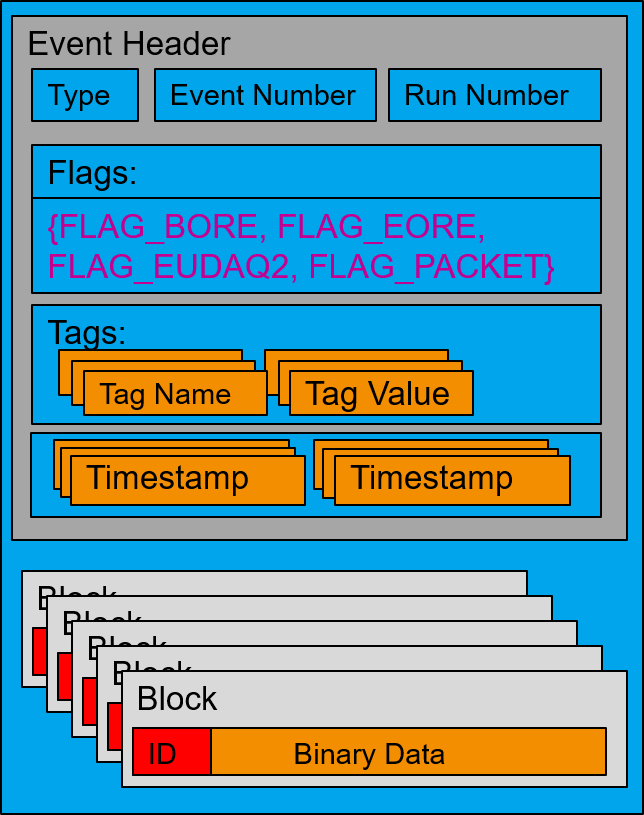
\includegraphics[width=.38\textwidth]{figures/rawdataevent.png}
	\caption[DAQ_System]{(A) Hardware and software layout of the DAQ system. (B) \rawdataevent}
	\label{fig:todo}
\end{figure}

% \begin{figure}[tb]
% 	\center
% 	
% 	\caption[DAQ_System]{\rawdataevent}
% 	\label{fig:todo}
% \end{figure}



The Run-Control is the central point for human interactions. 
From it the producer are configured, started, stopped and terminated. 
Currently there are two implementation of the Run-Control one command line version called TestRunControl and one GUI version Called euRun. 
Both have the about same functionality. 
The LogCollector receives all status/error messages that are produced by any of the producer. 
It has the possibility to filter for different warning levels. 
The DataCollector has a direct connection do all the producer. 
\eudaq 1.x is an event based DAQ system, therefore the Data-Collector expects that all producer send one event per trigger that they have reserved from the TLU. 
And that all events from different producer share a common trigger number by which they get merged into one container event called Detector-Event. 
The Data-collector has the possibility to do some basic sanity checks on the events like event number mismatch. 
The Producer handles the communication between the \eudaq framework and the user DAQ system. 
The user has to write its own Producer class which inherits from the abstract class producer. 
This class encapsulates the TCP/IP communication. 
The user needs to implement four virtual functions which handle the transit from one state to another. 
The producer has three states: unconfigured, configured and running. 
The configuration file is a plain text file which contains a section for each producer. 
Each sections contains tag-value pairs for the configuration of the producer. 
Sections for producer that are currently not connected are ignored. 
The basic event type that is used for user's data is the \rawdataevent. 
\rawdataevents are separated by the sub event type. 
A string which identifies the producer it belongs to. 
The sub event type is used to determine the corresponding data converter plugin. 
The \rawdataevent has the possibility to store tag value pairs as well as plain binary data. 
The ConverterPlugins are used to convert the data from plain binary data to pixels hits. 
The ConverterPlugin is explicitly not called from the DataCollector this makes it possible that the data collector can handle unknown data types. 
The \eudaq Framework comes with an online monitor which can either run online during the data taking or offline on files on disk. 
It produces hit-map and correlation-plots for all known producer types. 
